% Full instructions available at:
% https://github.com/elauksap/focus-beamertheme

\documentclass{beamer}
\usetheme{focus}

\title{LDpred2: better, faster, stronger }
\subtitle{Privé, Arbel, Vilhjálmsson;BiorXiv 2020}
\author{Discussion led by: Bárbara Bitarello}
%\titlegraphic{
\includegraphics[scale=1.25]{focuslogo.pdf}}
%\institute{Institute Name \\ Institute Address}
\date{02 - 07 - 2020}

\begin{document}
    \begin{frame}
        \maketitle
    \end{frame}
    
   \section{Background: LDpred}
   
   \begin{frame}
   \large Important background 
   
\includegraphics[width=100mm,scale=1]{daft_punk.png}
       
   \end{frame}
    \begin{frame}[t]{What does LDpred do?}
        Published in 2015:  $\sim$ 435 citations (less than PRSice from same year)
        \begin{itemize}

            \item matrix of correlation between genetic variants (LD matrix), summary statistics from GWAS ($\beta$, $p-value$), genotype and phenotype files from test and validation sets 
                \end{itemize}
                \begin{columns}[t, onlytextwidth]
            \column{0.45\textwidth}
    \textcolor{example}{Infinitesimal:}
    \begin{itemize}
        \item All markers are causal
        \item Effect sizes drawn from Gaussian
        \item  Computationally efficient
        \item Not very plausible 
    \end{itemize}
     \column{0.45\textwidth}
     \textcolor{example}{Non-infinitesimal}
    
   \begin{itemize}
    
    \item  Assumes \emph{p} of variants are causal - more plausible 
  
     \item Analytical solution hard - approximate MCMC Gibbs sampler (not efficient nor robust)
     \end{itemize}
     \end{columns}
    \end{frame}

%    \begin{frame}[plain]{Plain frame}
\begin{frame}[t]{What does LDpred do?}
But \emph{actually} also requires:
\begin{itemize}
        \item big LD reference panel, correct model specifications  - not trivial
        \item Steps:
            \begin{itemize}
                \item Coordinating summary stats, LD reference genotypes, validation or test genotypes
                \item Estimating weights for variants - which requires additional parameters.
                \item Calculating PRS 
                \item User needs to calculate partial-R\textsuperscript{2} on their own (e.g. in R)
        \end{itemize}
    \end{itemize}
\end{frame}

%next
   \begin{frame}{LDpred: pros and cons overview}
   \begin{columns}[t, onlytextwidth]
              \column{0.45\textwidth}
    \textcolor{example}{PROS:}
    \begin{itemize}
            \item elegant modelling of genetic architecture
            \item assigns weights to variants instead of arbitrary P+T
            \item also offers P+T in the same framework
            \item mostly runs PLINK in the background, and Python scripts
         \end{itemize}
                   \column{0.45\textwidth}
    \alert{CONS:} 
        \begin{itemize}
            \item Errors messages are cryptic
            \item \alert{Slow}
            \item Gibbs sampler \alert{extremely sensitive to model parameters}
            \item particularly bad for long-range LD regions (e.g HLA)
            \item MCMC setup might or not improve things and makes it it \emph{much slower}
            \item No manual available. 
            \end{itemize}
            \end{columns}
     \end{frame}
     
  \section{New method: LDpred2}   
  \begin{frame}{LDpred2: what's new?}
    \begin{itemize}
        \item Runs in bigsnpr package in \alert{R}. \alert{Better?}
        \item \alert{Faster}
        \item LDpred-auto: learns parameters from the data. \alert{Stronger}
        \item \alert{More accurate} PRS: simulation and real data benchmarking
        \item Compares favorably to other methods [sort of] 
        \item \alert{has tutorial}!! \alert{Better!} \url{https://privefl.github.io/bigsnpr/articles/LDpred2.html}
    \end{itemize}

  \end{frame}
    \begin{frame}[t]{Simulations: methods}
            Binary phenotypes; each set 10X (average AUC is reported)
        \begin{itemize}
         \item UKBB data
         \item unrelated individuals - 360K
          \begin{itemize}
                    \item 10,000 for validation, LD reference
                    \item 300,000 for GWAS
                    \item $\sim$ 52,000 as test set 
                    \end{itemize}
            
         \item HapMap3 variants - 1.1 Million

                  \item $h^2=0.4$ or $h^2=0.3$, prevalence 15\%
                  \item $M=\{300,3000,30000,300000\}$
                  \item Variance of genetic liability=$h^2$
                  \item HLA region
                  \item Implemented in bigsnpr
              \end{itemize}
    \end{frame}
    
 
  
    \begin{frame}[t]{Real data: methods}
       
          \begin{itemize}
                \item Unrelated individuals - 360K
                \item All case-control phenotypes
                \item 10,000 for validation, LD reference
                \item $\sim$ 352,000 as test set 
                \item Compare LDpred1, LDpred2, C+T, SCT, lassosum, PRS-CS
                \item summary statistics:
            \end{itemize}
                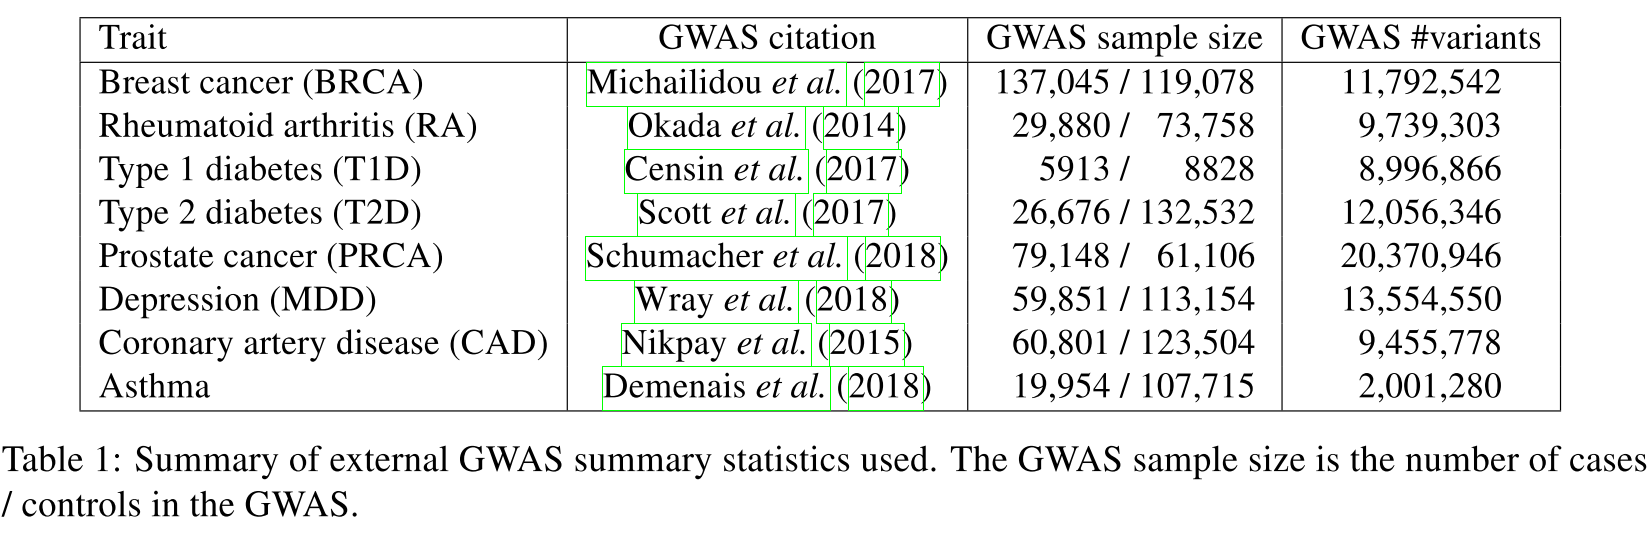
\includegraphics[width=120mm,scale=1.2]{table1.png}
    \end{frame}
    
      \begin{frame}[t]{Methods: performance comparisons}
         \begin{columns}[onlytextwidth]
              \column{0.45\textwidth}
                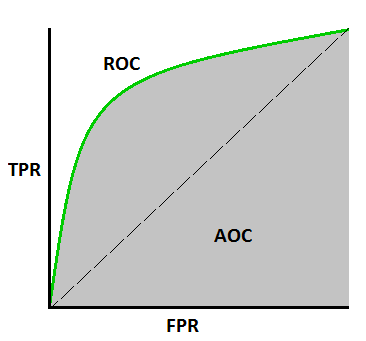
\includegraphics[width=60mm,scale=0.6]{auc.png}
                
                \column{0.35\textwidth}
                $TPR=\frac{TP}{TP+FN}$
                \newline
                \newline
                $Specificity=\frac{TN}{TN+FP}$
                \newline
                \newline
                $FPR=1-Specifcity$
                \end{columns}
                \vfill
                \tiny 
                Image: \url{https://towardsdatascience.com/understanding-auc-roc-curve-68b2303cc9c5}
     \end{frame}
%summary statistics
% high number of cases in UK Biobank (UKBB)
 
    \begin{frame}[t]{Simulations: Results}
    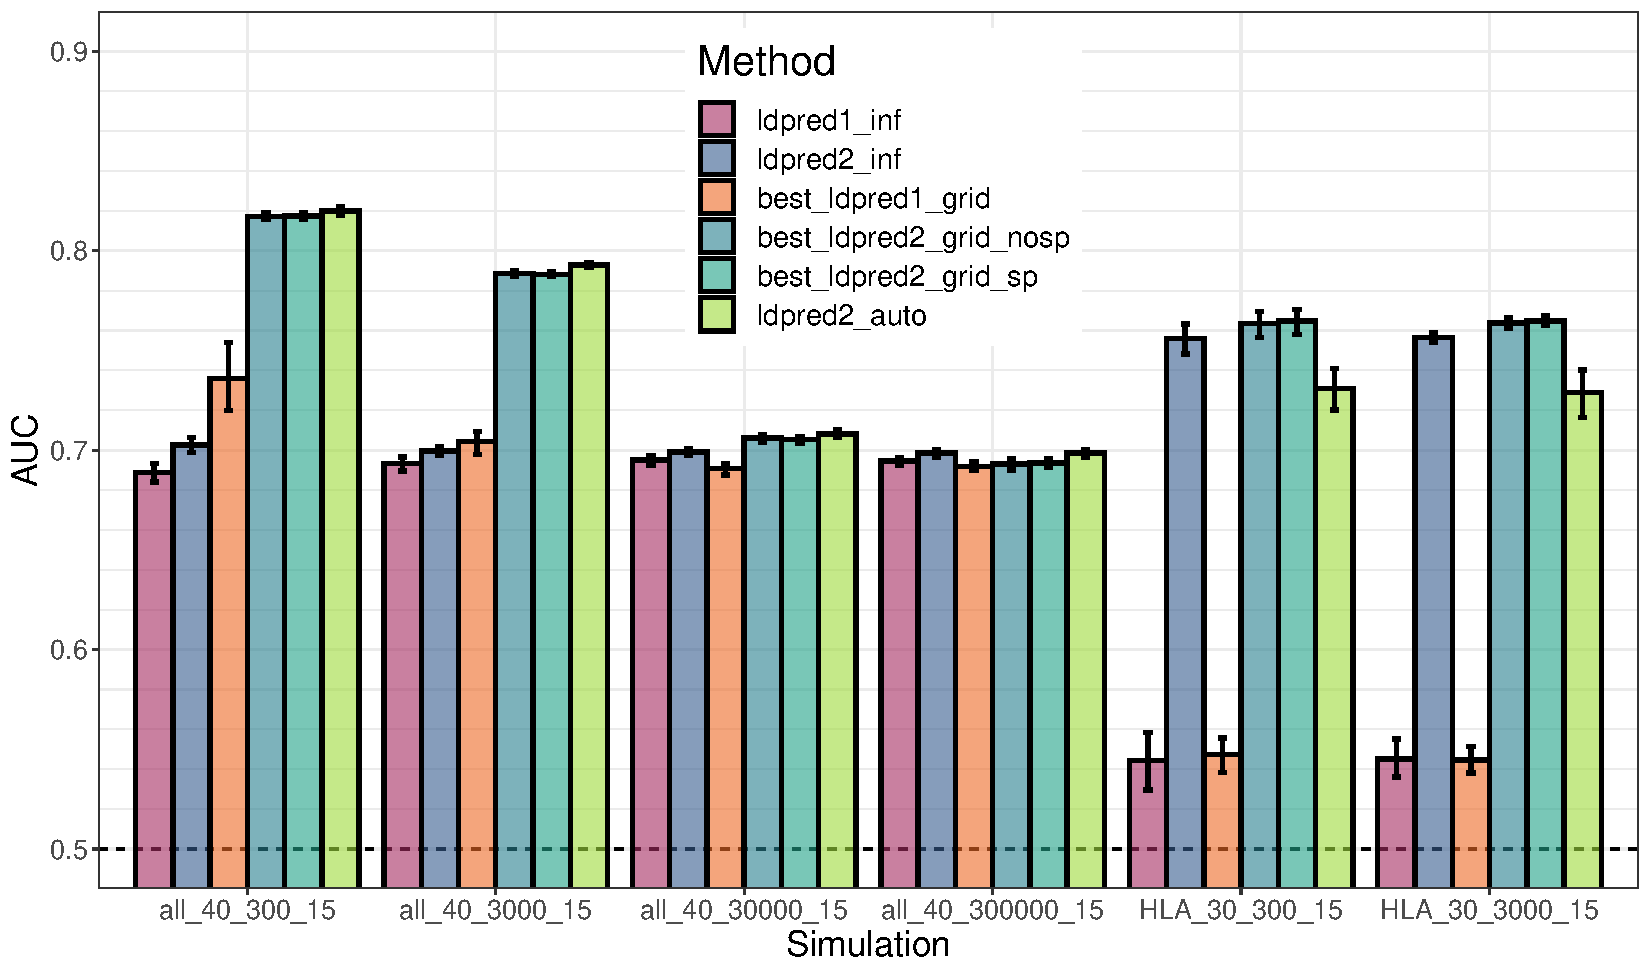
\includegraphics[width=100mm,scale=1]{AUC-simu.pdf}
 
      \end{frame}
      
   
       \begin{frame}[t]{Real Data: Results}
       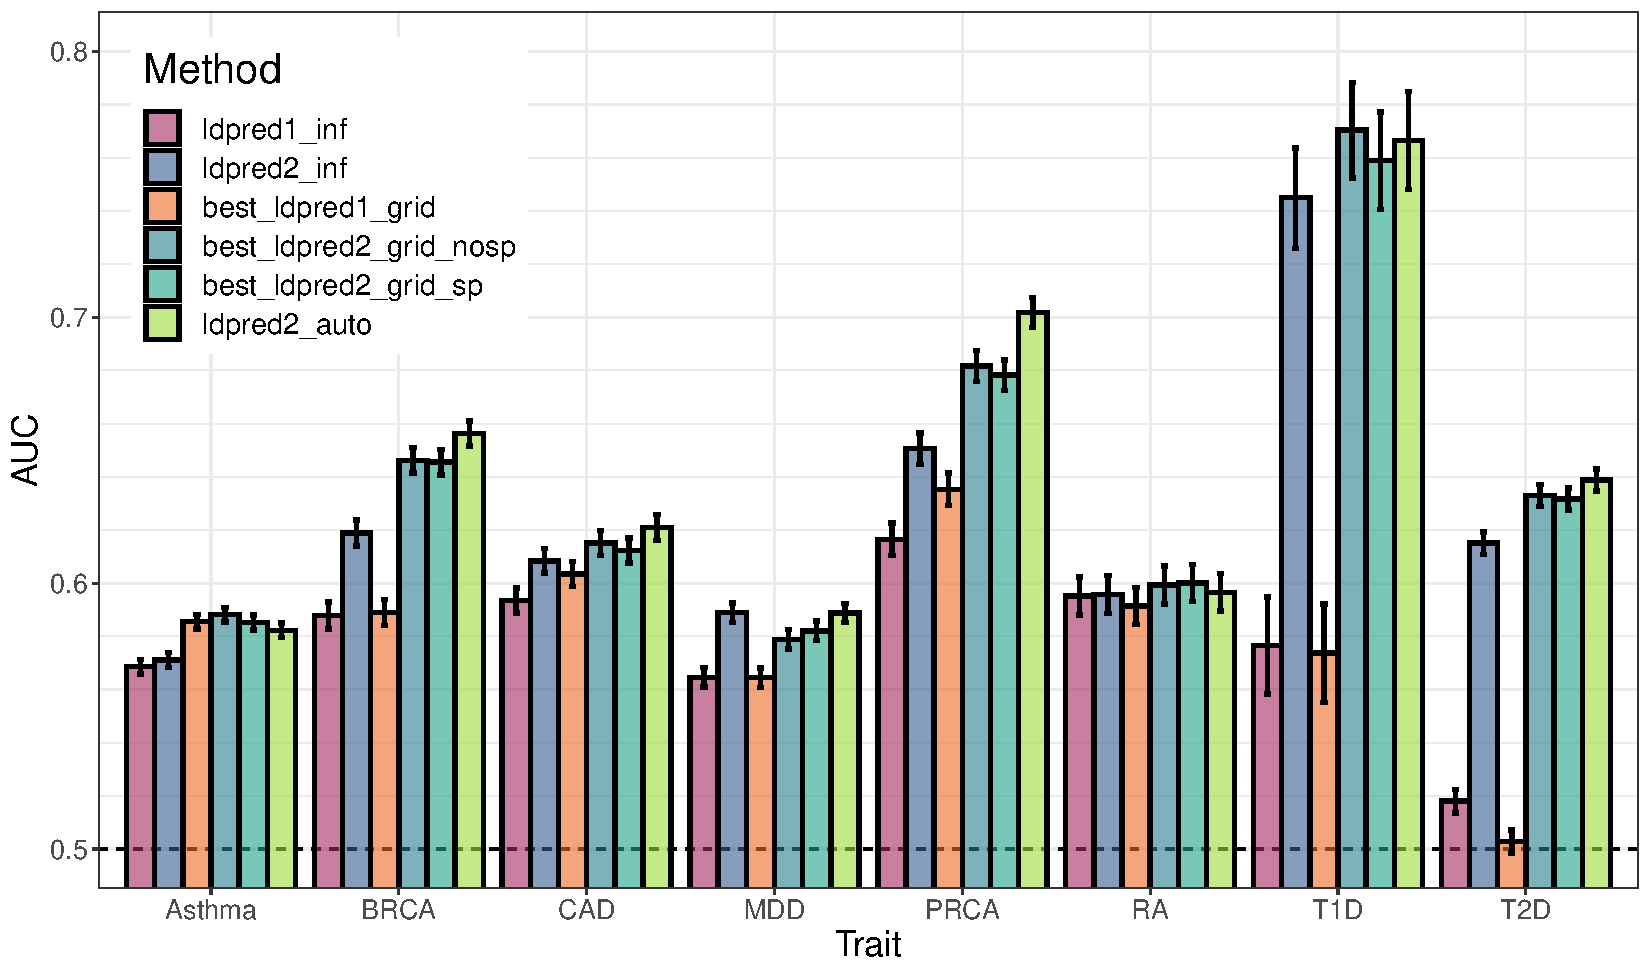
\includegraphics[width=100mm,scale=1]{AUC-real.pdf}
    \end{frame}
    
       \begin{frame}[t]{Real Data: Results}
       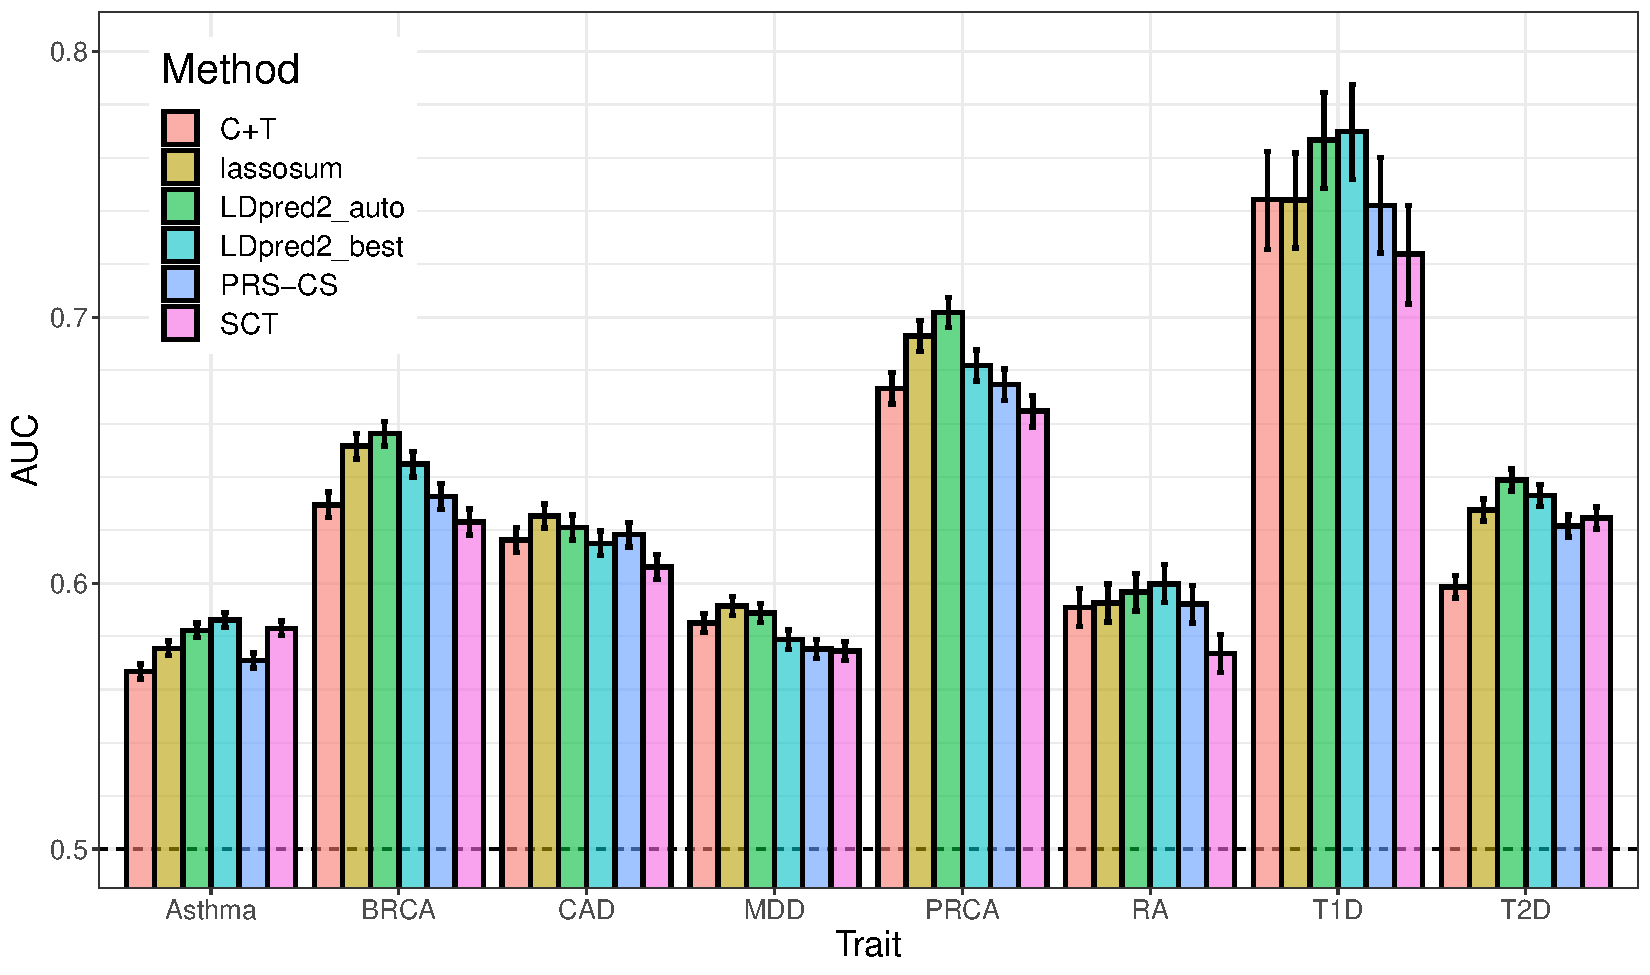
\includegraphics[width=100mm,scale=1]{AUC-all.pdf}
    \end{frame}
    
    
        
     \begin{frame}{Conclusions}
        \begin{itemize}
            \item Strengths: long-range LD and less polygenic traits, does not require validation step
            %to choose hyperparameters. What are they? they are parameters of a prior, which is itself used to pick parameters of the model.
            \item solves gibbs sampler inconsistencies
            \item higher prediction accuracy then LDpred1
            \item Use HapMap3 variants
           \newline
           \newline
            \item Not really better than lassosum?
            \item Still kinda slow
        \end{itemize}
       \end{frame}
    
    
    
    
  
    
%    \begin{frame}{Typesetting and Math}
%        The packages \texttt{inputenc} and \texttt{FiraSans}\footnote{\url{https://fonts.google.com/specimen/Fira+Sans}}\textsuperscript{,}\footnote{\url{http://mozilla.github.io/Fira/}} are used to properly set the main fonts.
%        \vfill
%        This theme provides styling commands to typeset \emph{emphasized}, \alert{alerted}, \textbf{bold}, \textcolor{example}{example text}, \dots
%       \vfill
%        \texttt{FiraSans} also provides support for mathematical symbols:
%        \begin{equation*}
%            e^{i\pi} + 1 = 0.
%        \end{equation*}
%    \end{frame}



%BLOCKS%%%%%
%    \section{Section 2}
%    \begin{frame}{Blocks}
%       \begin{block}{Block}
%            Text.
%        \end{block}
%        \pause
%        \begin{alertblock}{Alert block}
%            Alert \alert{text}.
%        \end{alertblock}
%        \pause
%        \begin{exampleblock}{Example block}
%            Example \textcolor{example}{text}.
%        \end{exampleblock}
%    \end{frame}

%LISTS

%    \begin{frame}{Lists}
%        \begin{columns}[t, onlytextwidth]
%            \column{0.33\textwidth}
%                Items:
%                \begin{itemize}
%                    \item Item 1
%                    \begin{itemize}
%                       \item Subitem 1.1
%                        \item Subitem 1.2
%                    \end{itemize}
%                    \item Item 2
%                    \item Item 3
%                \end{itemize}
%            
%            \column{0.33\textwidth}
%                Enumerations:
%                \begin{enumerate}
%                    \item First
%                    \item Second
%                    \begin{enumerate}
%                        \item Sub-first
%                        \item Sub-second
%                    \end{enumerate}
%                    \item Third
%                \end{enumerate}
%            
%            \column{0.33\textwidth}
%                Descriptions:
%                \begin{description}
%                    \item[First] Yes.
%                    \item[Second] No.
%                \end{description}
%        \end{columns}
%    \end{frame}
%\setbeamertemplate{caption}[numbered]
%    \begin{frame}{Figures and Tables}
%        \begin{columns}
%            \column{0.4\textwidth}
%                \begin{figure}
%                    \centering
%                    
\includegraphics{focuslogo.pdf}
%                    \caption{Figure caption.}
%                    \label{fig:focuslogo}
%                \end{figure}
%                
%           \column{0.6\textwidth}
%               \begin{table}
%                    \centering
%                    \begin{tabular}{rcc}
%                         & Heading 1 & Heading 2 \\\hline
%                        Row 1 & \(v_{11}\) & \(v_{12}\) \\
%                        Row 2 & \(v_{21}\) & \(v_{22}\) \\
%                        Row 3 & \(v_{31}\) & \(v_{32}\) \\
%                    \end{tabular}
%                   \caption{Table caption.}
%                    \label{tab:demo}
%                \end{table}
%        \end{columns}
%    \end{frame}
    
%    \begin{frame}[focus]
    %       Thanks for using \textbf{Focus}!
%    \end{frame}
    
    \appendix
%    \begin{frame}{References}
%        \nocite{*}
%        \bibliography{demo_bibliography}
%        \bibliographystyle{plain}
%    \end{frame}
    
    \begin{frame}[t]{LDpred model}
    Unlinked markers and non-infinitesimal architecture\\
    \newline
    
    Effects are drawn from a mixture distribution:
    \begin{equation}
 \beta_{i}\sim\begin{cases}
    N(0, \frac{h^2}{Mp}), & \text{with probability $p$}.\\
    0, & \text{with probability $1-p$}.
  \end{cases}
\end{equation}
        
        
    
    \end{frame}
    
       \begin{frame}{LDpred model}
       \end{frame}
       
       
       \begin{frame}{MCMC, Gibbs Sampler etc}
       \end{frame}
       
\end{document}
